\section{KL正则化的成本最小化}
\label{sec:dsel-kl-cost}

只降低期望成本，会把全部质量推到成本最低的状态上。若参考分布$P$代表原有的规律，我们愿意为降低成本而改动它，但改动本身也要付出代价。把这个代价记为$\tau D_{\mathrm{KL}}(Q\Vert P)$，$\tau>0$是一个换算系数：偏离参考分布一个nat，相当于多付$\tau$个单位的成本。

设$V:\mathcal{X}\to\mathbb{R}$可测，在每一点取有限值。在式~\eqref{eq:dsel-candidate-set}的候选集合上考虑
\begin{equation}
 \min_{Q\in\mathcal{Q}_V}\ J_\tau(Q),\qquad J_\tau(Q)=\mathbb{E}_{Q}[V]+\tau D_{\mathrm{KL}}(Q\Vert P).
 \label{eq:dsel-kl-cost-problem}
\end{equation}
在目标上加一个KL项以约束解不要离参考分布太远，这种做法称为\term{KL正则化}（KL regularization）。

\paragraph{有限状态上的权衡}
先在有限的$\mathcal{X}$上、$p(x)>0$处处成立时看目标的形状。这时
\[
 J_\tau(Q)=\sum_{x}q(x)V(x)+\tau\sum_{x}q(x)\ln\frac{q(x)}{p(x)} .
\]
第一项是线性的，它把质量拉向成本低的状态。第二项是凸的，而且函数$t\mapsto t\ln t$在$t\downarrow0$处的导数趋于$-\infty$：把某个状态的概率压到零，代价增长得极快。两者相抗，最优解应当留在三角形内部。

在内部，可以用归一化约束的Lagrange乘子$\nu$形式地求驻点。对$q(x)$求偏导并令其为零，得到
\[
 V(x)+\tau\Bigl(\ln\frac{q(x)}{p(x)}+1\Bigr)-\nu=0 .
\]
解出$q(x)$，
\[
 q(x)=p(x)\,\mathrm{e}^{-V(x)/\tau}\,\mathrm{e}^{\nu/\tau-1} .
\]
最后一个因子与$x$无关，由归一化确定。记$Z=\sum_xp(x)\mathrm{e}^{-V(x)/\tau}$，于是候选解是
\[
 q(x)=\frac{p(x)\,\mathrm{e}^{-V(x)/\tau}}{Z} .
\]
每个状态的参考概率乘上一个只由它自己的成本决定的权重$\mathrm{e}^{-V(x)/\tau}$，再整体归一。这一推导假设了解在内部且可微，只是猜测，下面将不借助导数直接验证它。

回到例子：$P$均匀，$V(x)=x$。取$\tau=1/\ln2$，权重就是$\mathrm{e}^{-V/\tau}=2^{-x}$，成本每多一个单位，权重减半。三个状态未归一的质量与归一化常数为
\[
 \frac13,\quad\frac16,\quad\frac1{12};\qquad Z=\frac13+\frac16+\frac1{12}=\frac7{12} .
\]
除以$Z$，得到
\[
 Q^{*}=\Bigl(\frac47,\ \frac27,\ \frac17\Bigr).
\]
图~\ref{fig:dsel-gibbs-bars}画出这一步：先乘权重，再归一化，质量从高成本状态挪向低成本状态，但没有任何状态被删去。

\begin{BookInlineFigure}
 \centering
 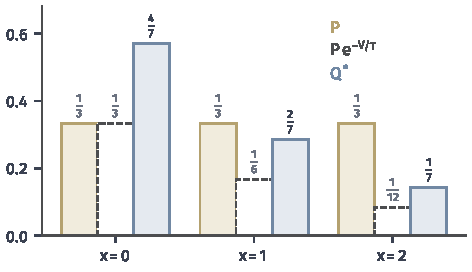
\includegraphics[width=80mm]{figures/07-probability/07-distribution-optimization/matplotlib/dsel-gibbs-bars/figure.pdf}
 \caption{按成本重新加权。$P$均匀（黄），$V(x)=x$，$\tau=1/\ln2$。白色虚线柱是未归一的$P\,\mathrm{e}^{-V/\tau}$，和为$Z=7/12$；蓝色柱是归一化后的$Q^{*}=(\frac47,\frac27,\frac17)$。}
 \label{fig:dsel-gibbs-bars}
\end{BookInlineFigure}

验证这个分布确实比别的好，先算它的目标值。期望成本是
\[
 \mathbb{E}_{Q^{*}}[V]=0\cdot\frac47+1\cdot\frac27+2\cdot\frac17=\frac47 .
\]
$P$的每个概率都是$1/3$，所以对数比是$\ln(3q^{*}(x))$，KL项为
\[
 D_{\mathrm{KL}}(Q^{*}\Vert P)=\frac47\ln\frac{12}7+\frac27\ln\frac67+\frac17\ln\frac37\approx0.3080-0.0440-0.1210=0.1429 .
\]
乘以$\tau=1/\ln2$后，KL项约为$0.2062$，相当于以比特计的偏离量。两项相加，
\[
 J_\tau(Q^{*})\approx0.5714+0.2062=0.7776 .
\]
对照两个极端：$\delta_0$的成本为零但偏离为$\ln3$，$P$的偏离为零但成本为$1$，
\[
 J_\tau(\delta_0)=\log_23\approx1.585,\qquad J_\tau(P)=1 .
\]
两者都比$Q^{*}$差。

\paragraph{参数$\tau$的作用}
$\tau$越小，偏离越便宜，解越接近只看成本的答案；$\tau$越大，偏离越贵，解越接近$P$。在例子中，$Q^{*}_\tau\propto\mathrm{e}^{-x/\tau}$。$\tau=0.5$时它约为$(0.867,0.117,0.016)$，$\tau=4$时约为$(0.419,0.326,0.254)$。$\tau\to0$时，权重$\mathrm{e}^{-x/\tau}$在$x=1,2$处趋于零，在$x=0$处恒为$1$，所以$Q^{*}_\tau\to\delta_0$；$\tau\to\infty$时三个权重都趋于$1$，$Q^{*}_\tau\to P$。图~\ref{fig:dsel-gibbs-path}画出这条从$\delta_0$到$P$的路径。

\begin{BookInlineFigure}
 \centering
 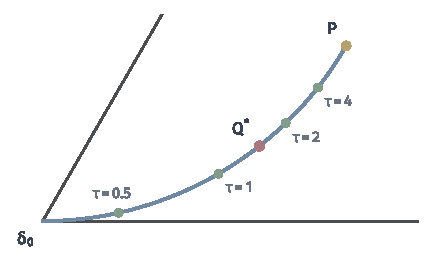
\includegraphics[width=72mm]{figures/07-probability/07-distribution-optimization/matplotlib/dsel-gibbs-path/figure.pdf}
 \caption{$\tau$从$0$增大到$\infty$时，$Q^{*}_\tau\propto P\,\mathrm{e}^{-V/\tau}$在概率三角形左下部分走过的路径（蓝），$P$均匀，$V(x)=x$。绿点依次是$\tau=0.5,1,2,4$，红点是$\tau=1/\ln2$时的$(\frac47,\frac27,\frac17)$，黄点是$P$。}
 \label{fig:dsel-gibbs-path}
\end{BookInlineFigure}

换一个角度看这个权衡。每个候选$Q$对应平面上的一点，横坐标是偏离$D_{\mathrm{KL}}(Q\Vert P)$，纵坐标是期望成本$\mathbb{E}_{Q}[V]$。目标$J_\tau$的等值线是斜率为$-\tau$的直线
\[
 \mathbb{E}_{Q}[V]=c-\tau D_{\mathrm{KL}}(Q\Vert P) .
\]
最小化$J_\tau$，就是把这条直线向下平移，直到它刚好碰到所有候选点组成的区域。图~\ref{fig:dsel-tradeoff}中，碰到的点正是$Q^{*}$；不同的$\tau$给出不同的斜率，碰到区域下边界上不同的点，而整条下边界就是上面那条Gibbs路径。下面的定理会证明这一点。

\begin{BookInlineFigure}
 \centering
 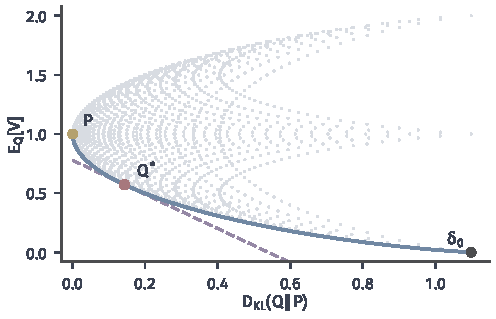
\includegraphics[width=84mm]{figures/07-probability/07-distribution-optimization/matplotlib/dsel-tradeoff/figure.pdf}
 \caption{成本与偏离的权衡，$P$均匀，$V(x)=x$。浅灰点是概率三角形中步长$1/60$的格点分布对应的$\bigl(D_{\mathrm{KL}}(Q\Vert P),\mathbb{E}_{Q}[V]\bigr)$；蓝线是Gibbs路径，它是可达区域的下边界。紫色虚线是$\tau=1/\ln2$时目标的等值线$\mathbb{E}_{Q}[V]=J^{*}-\tau D_{\mathrm{KL}}(Q\Vert P)$，在红点$Q^{*}$处与边界相切。}
 \label{fig:dsel-tradeoff}
\end{BookInlineFigure}

\paragraph{Gibbs分布的最优性}
有限状态上的形式推导提示了一般的答案：把$P$按$\mathrm{e}^{-V/\tau}$重新加权。下面在一般可测空间上定义它，并直接证明它的最优性。

\begin{definition}[Gibbs分布]
\label{def:dsel-gibbs}
设$P\in\mathcal{P}(\mathcal{X})$，$V:\mathcal{X}\to\mathbb{R}$可测，$\tau>0$，且
\begin{equation}
 Z=\mathbb{E}_{P}\bigl[\mathrm{e}^{-V/\tau}\bigr]<\infty .
 \label{eq:dsel-gibbs-partition}
\end{equation}
以
\begin{equation}
 \frac{\mathrm{d}Q^{*}_\tau}{\mathrm{d}P}=\frac{\mathrm{e}^{-V/\tau}}{Z}
 \label{eq:dsel-gibbs}
\end{equation}
定义的概率测度$Q^{*}_\tau$称为成本$V$、参数$\tau$相对于$P$的\term{Gibbs分布}（Gibbs distribution）。
\end{definition}

被积函数$\mathrm{e}^{-V/\tau}$处处为正，所以$Z>0$总成立，式~\eqref{eq:dsel-gibbs-partition}中真正的条件是$Z$有限。密度$\mathrm{e}^{-V/\tau}/Z$处处为正且有限，因此$Q^{*}_\tau$与$P$互相绝对连续：二者的零概率事件完全相同。

\begin{theorem}[Gibbs变分原理]
\label{thm:dsel-gibbs-variational}
设$V:\mathcal{X}\to\mathbb{R}$可测，$\tau>0$，$Z=\mathbb{E}_{P}[\mathrm{e}^{-V/\tau}]<\infty$，$Q^{*}=Q^{*}_\tau$为式~\eqref{eq:dsel-gibbs}的Gibbs分布。
\begin{enumerate}
 \item 对每个$Q\in\mathcal{Q}_V$，
 \begin{equation}
 J_\tau(Q)=-\tau\ln Z+\tau D_{\mathrm{KL}}(Q\Vert Q^{*}) .
 \label{eq:dsel-gibbs-identity}
 \end{equation}
 特别地，$J_\tau(Q)\geq-\tau\ln Z$。
 \item 若还有$\mathbb{E}_{Q^{*}}\lvert V\rvert<\infty$，则$Q^{*}\in\mathcal{Q}_V$，$J_\tau(Q^{*})=-\tau\ln Z$，并且$Q^{*}$是问题~\eqref{eq:dsel-kl-cost-problem}的唯一最优分布。
\end{enumerate}
\end{theorem}

\begin{proof}
第一部分。设$Q\in\mathcal{Q}_V$。由$D_{\mathrm{KL}}(Q\Vert P)<\infty$知$Q\ll P$；$P$与$Q^{*}$互相绝对连续，所以$Q\ll Q^{*}$。由密度的链式法则与式~\eqref{eq:dsel-gibbs}，$Q$几乎处处有
\[
 \frac{\mathrm{d}Q}{\mathrm{d}Q^{*}}=\frac{\mathrm{d}Q}{\mathrm{d}P}\cdot\frac{\mathrm{d}P}{\mathrm{d}Q^{*}}=\frac{\mathrm{d}Q}{\mathrm{d}P}\cdot Z\,\mathrm{e}^{V/\tau} .
\]
取对数，
\[
 \ln\frac{\mathrm{d}Q}{\mathrm{d}Q^{*}}=\ln\frac{\mathrm{d}Q}{\mathrm{d}P}+\frac{V}{\tau}+\ln Z .
\]

右边每一项都在$Q$下可积：$D_{\mathrm{KL}}(Q\Vert P)$有限，而对数比的负部总是可积的，所以$\ln(\mathrm{d}Q/\mathrm{d}P)$在$Q$下可积；$V$在$Q$下可积是$\mathcal{Q}_V$的定义；$\ln Z$是常数。于是可以对右边逐项取$Q$下的期望，左边的期望就是$D_{\mathrm{KL}}(Q\Vert Q^{*})$：
\[
 D_{\mathrm{KL}}(Q\Vert Q^{*})=D_{\mathrm{KL}}(Q\Vert P)+\frac{1}{\tau}\mathbb{E}_{Q}[V]+\ln Z .
\]
两边乘以$\tau$并移项，即得式~\eqref{eq:dsel-gibbs-identity}。由Gibbs不等式$D_{\mathrm{KL}}(Q\Vert Q^{*})\geq0$，得到$J_\tau(Q)\geq-\tau\ln Z$。

第二部分。由式~\eqref{eq:dsel-gibbs}，$\ln(\mathrm{d}Q^{*}/\mathrm{d}P)=-V/\tau-\ln Z$。当$V$在$Q^{*}$下可积时，它在$Q^{*}$下可积，
\[
 D_{\mathrm{KL}}(Q^{*}\Vert P)=-\frac1\tau\mathbb{E}_{Q^{*}}[V]-\ln Z<\infty ,
\]
所以$Q^{*}\in\mathcal{Q}_V$。在式~\eqref{eq:dsel-gibbs-identity}中取$Q=Q^{*}$，得到$J_\tau(Q^{*})=-\tau\ln Z$，它等于第一部分给出的下界，所以$Q^{*}$最优。若另一个$Q\in\mathcal{Q}_V$也达到这个值，则$D_{\mathrm{KL}}(Q\Vert Q^{*})=0$，由Gibbs不等式的等号条件$Q=Q^{*}$。
\end{proof}

定理~\ref{thm:dsel-gibbs-variational}称为\term{Gibbs变分原理}（Gibbs variational principle）。式~\eqref{eq:dsel-gibbs-identity}比“$Q^{*}$最优”说得更多：任何候选的目标值比最优值多出的部分，恰好是$\tau D_{\mathrm{KL}}(Q\Vert Q^{*})$。在例子中，$J_\tau(P)-J_\tau(Q^{*})\approx1-0.7776=0.2224$，而直接计算
\[
 \tau D_{\mathrm{KL}}(P\Vert Q^{*})=\frac{1}{3\ln2}\ln\Bigl(\frac{7}{12}\cdot\frac76\cdot\frac73\Bigr)=\frac13\log_2\frac{343}{216}\approx0.2224 ,
\]
两者一致。这个恒等式把“离最优还差多少”变成一个可以计算的散度，第~\ref{sec:dsel-checks}节将用它检验数值解。

最优值$-\tau\ln\mathbb{E}_{P}[\mathrm{e}^{-V/\tau}]$也有清楚的含义。令$g=-V/\tau$，第一部分可以改写为：对每个$Q\in\mathcal{Q}_V$，
\begin{equation}
 \mathbb{E}_{Q}[g]\leq D_{\mathrm{KL}}(Q\Vert P)+\ln\mathbb{E}_{P}\bigl[\mathrm{e}^{g}\bigr] ,
 \label{eq:dsel-dv}
\end{equation}
第~\ref{chap:distribution-comparison}章用这个不等式由KL散度控制期望差。定理的第二部分说明它不能再改进：当$\mathbb{E}_{Q^{*}}\lvert g\rvert<\infty$时，等号在指数倾斜$Q^{*}$处取到，于是
\[
 \ln\mathbb{E}_{P}\bigl[\mathrm{e}^{g}\bigr]=\max_{Q\in\mathcal{Q}_V}\Bigl\{\mathbb{E}_{Q}[g]-D_{\mathrm{KL}}(Q\Vert P)\Bigr\} .
\]
对数矩母函数是“期望减去偏离代价”在全体候选上的最大值。

Gibbs分布的形式不是事先选定的分布族，而是由目标推出来的。它是$P$沿统计量$V$、以参数$-1/\tau$作的指数倾斜，属于第~\ref{chap:distribution-families}章以$P$为基准测度、以$V$为自然统计量的指数族。

由定理还可以读出图~\ref{fig:dsel-tradeoff}中的下边界。设$Q\in\mathcal{Q}_V$的偏离不超过$Q^{*}$的偏离，即
\[
 D_{\mathrm{KL}}(Q\Vert P)\leq D_{\mathrm{KL}}(Q^{*}\Vert P) .
\]
由$J_\tau(Q)\geq J_\tau(Q^{*})$，
\[
 \begin{aligned}
 \mathbb{E}_{Q}[V]&\geq\mathbb{E}_{Q^{*}}[V]+\tau\bigl(D_{\mathrm{KL}}(Q^{*}\Vert P)-D_{\mathrm{KL}}(Q\Vert P)\bigr)\\
 &\geq\mathbb{E}_{Q^{*}}[V] .
 \end{aligned}
\]
也就是说，在不超过$Q^{*}$的偏离预算下，没有哪个分布的期望成本更低。

\paragraph{配分函数无穷时}
条件$Z<\infty$不是技术细节。回到第~\ref{sec:dsel-problems}节的可数例子：$P(k)=2^{-k}$，$V(k)=-k$，$k\geq1$。记$r=\mathrm{e}^{1/\tau}/2$，则
\[
 Z(\tau)=\sum_{k\geq1}2^{-k}\mathrm{e}^{k/\tau}=\sum_{k\geq1}r^{k} .
\]
它有限当且仅当$r<1$，即$\tau>1/\ln2$；这时$Z=r/(1-r)$，Gibbs分布$Q^{*}(k)=(1-r)r^{k-1}$是几何分布，$\mathbb{E}_{Q^{*}}\lvert V\rvert=1/(1-r)$有限，定理~\ref{thm:dsel-gibbs-variational}的两部分都适用。例如$\tau=2$时，$r\approx0.8244$，$Z\approx4.693$，最优值$-2\ln Z\approx-3.092$。

$\tau\leq1/\ln2$时没有Gibbs分布，最优值是$-\infty$。取$Q_N$为$\{1,\dots,N\}$上的均匀分布，它的期望成本与KL散度分别是
\[
 \begin{gathered}
 \mathbb{E}_{Q_N}[V]=-\frac{N+1}{2},\\
 D_{\mathrm{KL}}(Q_N\Vert P)=\frac1N\sum_{k=1}^{N}\bigl(k\ln2-\ln N\bigr)=\frac{(N+1)\ln2}{2}-\ln N .
 \end{gathered}
\]
代入目标，
\[
 J_\tau(Q_N)=\frac{N+1}{2}\bigl(\tau\ln2-1\bigr)-\tau\ln N .
\]
$\tau\ln2\leq1$时第一项不为正，第二项趋于$-\infty$，所以$J_\tau(Q_N)\to-\infty$。远处状态带来的收益$k$增长得不比偏离的代价$\tau k\ln2$慢，把质量往远处推永远划算。图~\ref{fig:dsel-partition-threshold}画出这一转变。

\begin{BookInlineFigure}
 \centering
 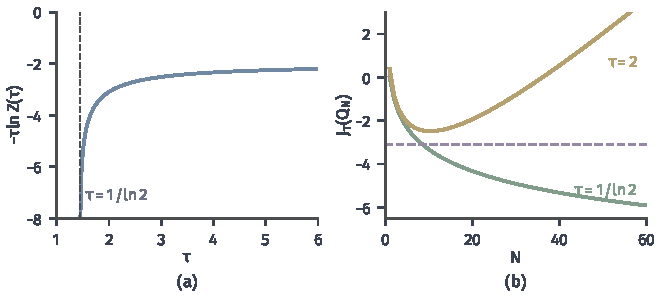
\includegraphics[width=112mm]{figures/07-probability/07-distribution-optimization/matplotlib/dsel-partition-threshold/figure.pdf}
 \caption{配分函数的有限性。$P(k)=2^{-k}$，$V(k)=-k$。(a)最优值$-\tau\ln Z(\tau)$（蓝），$\tau\downarrow1/\ln2$（深灰虚线）时趋于$-\infty$。(b)$\{1,\dots,N\}$上均匀分布$Q_N$的目标值：$\tau=1/\ln2$时（绿）等于$-\log_2N$，无下界；$\tau=2$时（黄）始终高于最优值$-2\ln Z(2)\approx-3.092$（紫色虚线）。}
 \label{fig:dsel-partition-threshold}
\end{BookInlineFigure}

定理第二部分的条件$\mathbb{E}_{Q^{*}}\lvert V\rvert<\infty$也可能不成立。那时$Z$有限，第一部分的恒等式仍然给出下界$-\tau\ln Z$，可是写出来的$Q^{*}$不在候选集合中。这种情形放到第~\ref{sec:dsel-checks}节，与“最小值是否被达到”一起讨论。
